\chapter{MST - Minimum Spanning Tree}

\section{Definizione}
\begin{itemize}
    \item Sia $G = (V,E)$ un grafo non orientato e connesso
    \item Sia $w : E \to R^+$
\end{itemize}

Un MST è $(V,T)$ con $T \subseteq E$ tale che:
\begin{itemize}
    \item $(V,T)$ è un albero (quindi $(V,T)$ è connesso e aciclico)
    \item $w(t) = \min_{\substack{A \subseteq E \text{ con } (V,A) \text{ albero}}}\{w(A)\}$
\end{itemize}

\subsection{Esempio}
\begin{center}
% ================= RIGA SUPERIORE =================
\begin{minipage}[c]{0.20\textwidth}
  \centering
  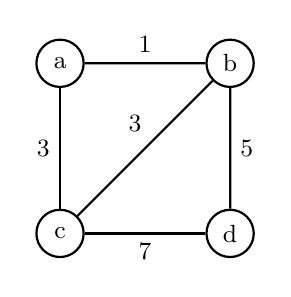
\begin{tikzpicture}[
      scale=1.2,
      node/.style={circle, draw=black, thick, fill=white, inner sep=0pt, minimum size=6mm, font=\small}
    ]
    % Nodi
    \node[node] (a) at (0, 1.8) {a};
    \node[node] (b) at (1.8, 1.8) {b};
    \node[node] (c) at (0, 0) {c};
    \node[node] (d) at (1.8, 0) {d};

    % Archi e pesi
    \draw[thick] (a) -- node[above] {\small $1$} (b);
    \draw[thick] (a) -- node[left]  {\small $3$} (c);
    \draw[thick] (c) -- node[above left, pos=0.55] {\small $3$} (b);
    \draw[thick] (b) -- node[right] {\small $5$} (d);
    \draw[thick] (c) -- node[below] {\small $7$} (d);
  \end{tikzpicture}
\end{minipage}%
\hfill
\begin{minipage}[c]{0.22\textwidth}
  \centering
  $\begin{aligned}
    \omega(a,b) &= 1 \\
    \omega(a,c) &= 3 \\
    &\;\;\vdots \\
    \omega(c,d) &= 7
  \end{aligned}$
\end{minipage}%
\hfill
\begin{minipage}[c]{0.20\textwidth}
  \centering
  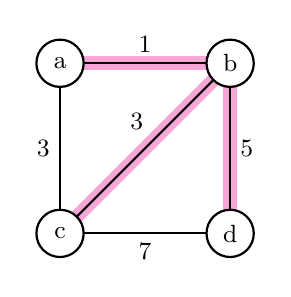
\begin{tikzpicture}[
      scale=1.2,
      node/.style={circle, draw=black, thick, fill=white, inner sep=0pt, minimum size=6mm, font=\small}
    ]
    % Nodi
    \coordinate (a) at (0, 1.8);
    \coordinate (b) at (1.8, 1.8);
    \coordinate (c) at (0, 0);
    \coordinate (d) at (1.8, 0);

    % Evidenziazione albero T (spessa e rosa)
    \draw[magenta!35, line width=5pt, line cap=round] (a) -- (b);
    \draw[magenta!35, line width=5pt, line cap=round] (c) -- (b);
    \draw[magenta!35, line width=5pt, line cap=round] (b) -- (d);

    % Archi e pesi
    \draw[thick] (a) -- node[above] {\small $1$} (b);
    \draw[thick] (a) -- node[left]  {\small $3$} (c);
    \draw[thick] (c) -- node[above left, pos=0.55] {\small $3$} (b);
    \draw[thick] (b) -- node[right] {\small $5$} (d);
    \draw[thick] (c) -- node[below] {\small $7$} (d);

    % Ridisegno nodi sopra gli archi
    \node[node] at (a) {a};
    \node[node] at (b) {b};
    \node[node] at (c) {c};
    \node[node] at (d) {d};
  \end{tikzpicture}
\end{minipage}%
\hfill
\begin{minipage}[c]{0.35\textwidth}
  $\begin{aligned}
    &T = \{(a,b),\, (b,c),\, (b,d)\} \quad (V,T) \text{ è un albero} \\
    &\omega(T) = 1 + 3 + 5 = 9 \\
    &T \text{ è a peso minimo} \\
    &\implies (V,T) \text{ è un MST}
  \end{aligned}$
\end{minipage}

\vspace{1.5em}

% ================= RIGA INFERIORE =================
\begin{minipage}[c]{0.20\textwidth}
  \centering
  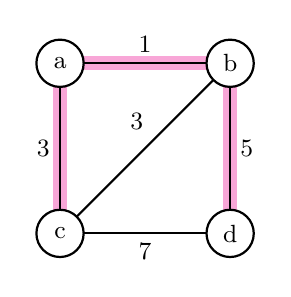
\begin{tikzpicture}[
      scale=1.2,
      node/.style={circle, draw=black, thick, fill=white, inner sep=0pt, minimum size=6mm, font=\small}
    ]
    % Nodi
    \coordinate (a) at (0, 1.8);
    \coordinate (b) at (1.8, 1.8);
    \coordinate (c) at (0, 0);
    \coordinate (d) at (1.8, 0);

    % Evidenziazione albero T' (spessa e rosa)
    \draw[magenta!35, line width=5pt, line cap=round] (a) -- (b);
    \draw[magenta!35, line width=5pt, line cap=round] (a) -- (c);
    \draw[magenta!35, line width=5pt, line cap=round] (b) -- (d);

    % Archi e pesi
    \draw[thick] (a) -- node[above] {\small $1$} (b);
    \draw[thick] (a) -- node[left]  {\small $3$} (c);
    \draw[thick] (c) -- node[above left, pos=0.55] {\small $3$} (b);
    \draw[thick] (b) -- node[right] {\small $5$} (d);
    \draw[thick] (c) -- node[below] {\small $7$} (d);

    % Ridisegno nodi sopra gli archi
    \node[node] at (a) {a};
    \node[node] at (b) {b};
    \node[node] at (c) {c};
    \node[node] at (d) {d};
  \end{tikzpicture}
\end{minipage}%
\hspace{0.04\textwidth}
\begin{minipage}[c]{0.70\textwidth}
  $\begin{aligned}
    &T' = \{(a,b),\, (a,c),\, (b,d)\} \\
    &\text{anche } (V,T') \text{ è un MST}
  \end{aligned}$
\end{minipage}
\end{center}

\subsection{Importanza di saper calcolare un MST}
\begin{itemize}
    \item Costruire reti eletteriche / idriche / \dots di minor costo possibile
    \item Collegare computer in un data center minimizzando la lunghezza dei cavi
    \item Clustering gerarchico
    \item Approssimizzazioni di problemi hard (TSP)
    \item Construire MST virtuali per l'instradamento
    \item Ottimizzare consumi energetici in sensori IoT
    \item Definire alveri di distribuzione in protocolli di rete
\end{itemize}

\newpage
\section{Come calcolare un MST}

\subsection{Requisiti}
Basta ricordare che $(V,A)$ è un albero (cioè è connesso e aciclico) se e solo se:
\begin{itemize}
    \item $(V,A)$ è connesso e $|A| = |V| - 1$
    \item $(V,A)$ è aciclico e $|A| = |V| - 1$
    \item $(V,A)$ è aciclico è massimale (se si aggiunge un arco ad $A$ si forma un ciclo)
\end{itemize}

\subsection{Procedimento}
\begin{itemize}
    \item 
\end{itemize}

\subsection{Pseudocodice}